\chapter{Linear Discriminant Analysis}
\label{chapter:pca}
\section{簡介}
\label{sec:background}




%Linear Discriminant Analysis(LDA),是一種降維演算法,但與前一節提到的PCA有些許的不同,這個演算法屬於一種「監督式」的學習法,所以在進行演算法的運算時,須考慮資料的類別。
Linear Discriminant Analysis(LDA),屬於一種「監督式」的降維演算法,所以在進行演算法運算時,須考慮資料的類別。
前一小節提到PCA是希望能在特徵空間中找到一個向量,使得資料的投影點,彼此之間的變異數越大越好。而LDA則是希望能夠找到一個投影向量,使得組內的離散程度越小越好,與組間的離散程度越大越好。


%\begin{figure}[h]
%	\centering
%	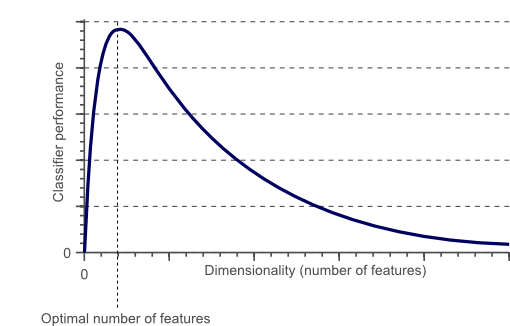
\includegraphics[height=5cm]{./pic/NZgacRXF.png}
%	\caption{維度災難示意圖}
%	\label{fig:curse_of_dimesionality}
%\end{figure}


\section{實例說明}
為了更簡單理解這個演算法的數學義意,以下舉一個例子說明:



\begin{itemize}
	\item
	      圖\ref{fig:pca_demostrate}為一個具有兩個維度的資料分佈圖。
	      \begin{figure}[h]
		      \centering
		      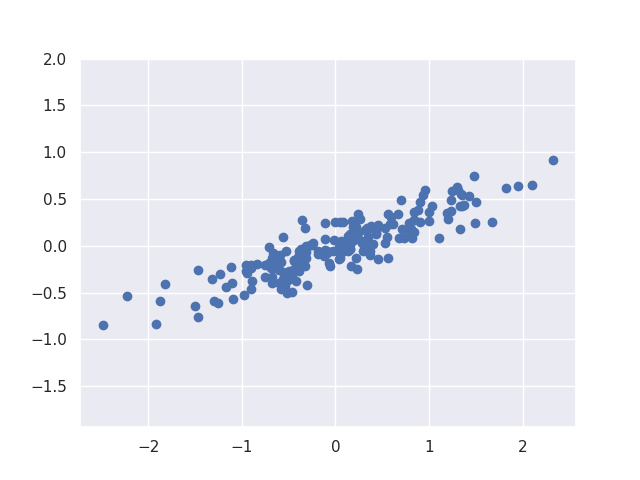
\includegraphics[width=9cm]{pic/pca_demostrate.png}
		      \caption{二維資料}
		      \label{fig:pca_demostrate}


	      \end{figure}


	      %
	\item
	      而PCA這個演算法的目的就是希望從這些資料點中如圖\ref{fig:pca_vector_to_find},找出投影向量,使得這些資料點投影在這些向量上後具有最大的變異數\footnote{\noindent 變異數:為對數據的變異程度的衡量,常用來量測資料分散程度之指標值,變異數其定義為 \(\sigma^2=\frac{{}\sum^{N}_{i}(x_i-\mu )^2}{N}\) }。
	      \begin{figure}[h]
		      \centering
		      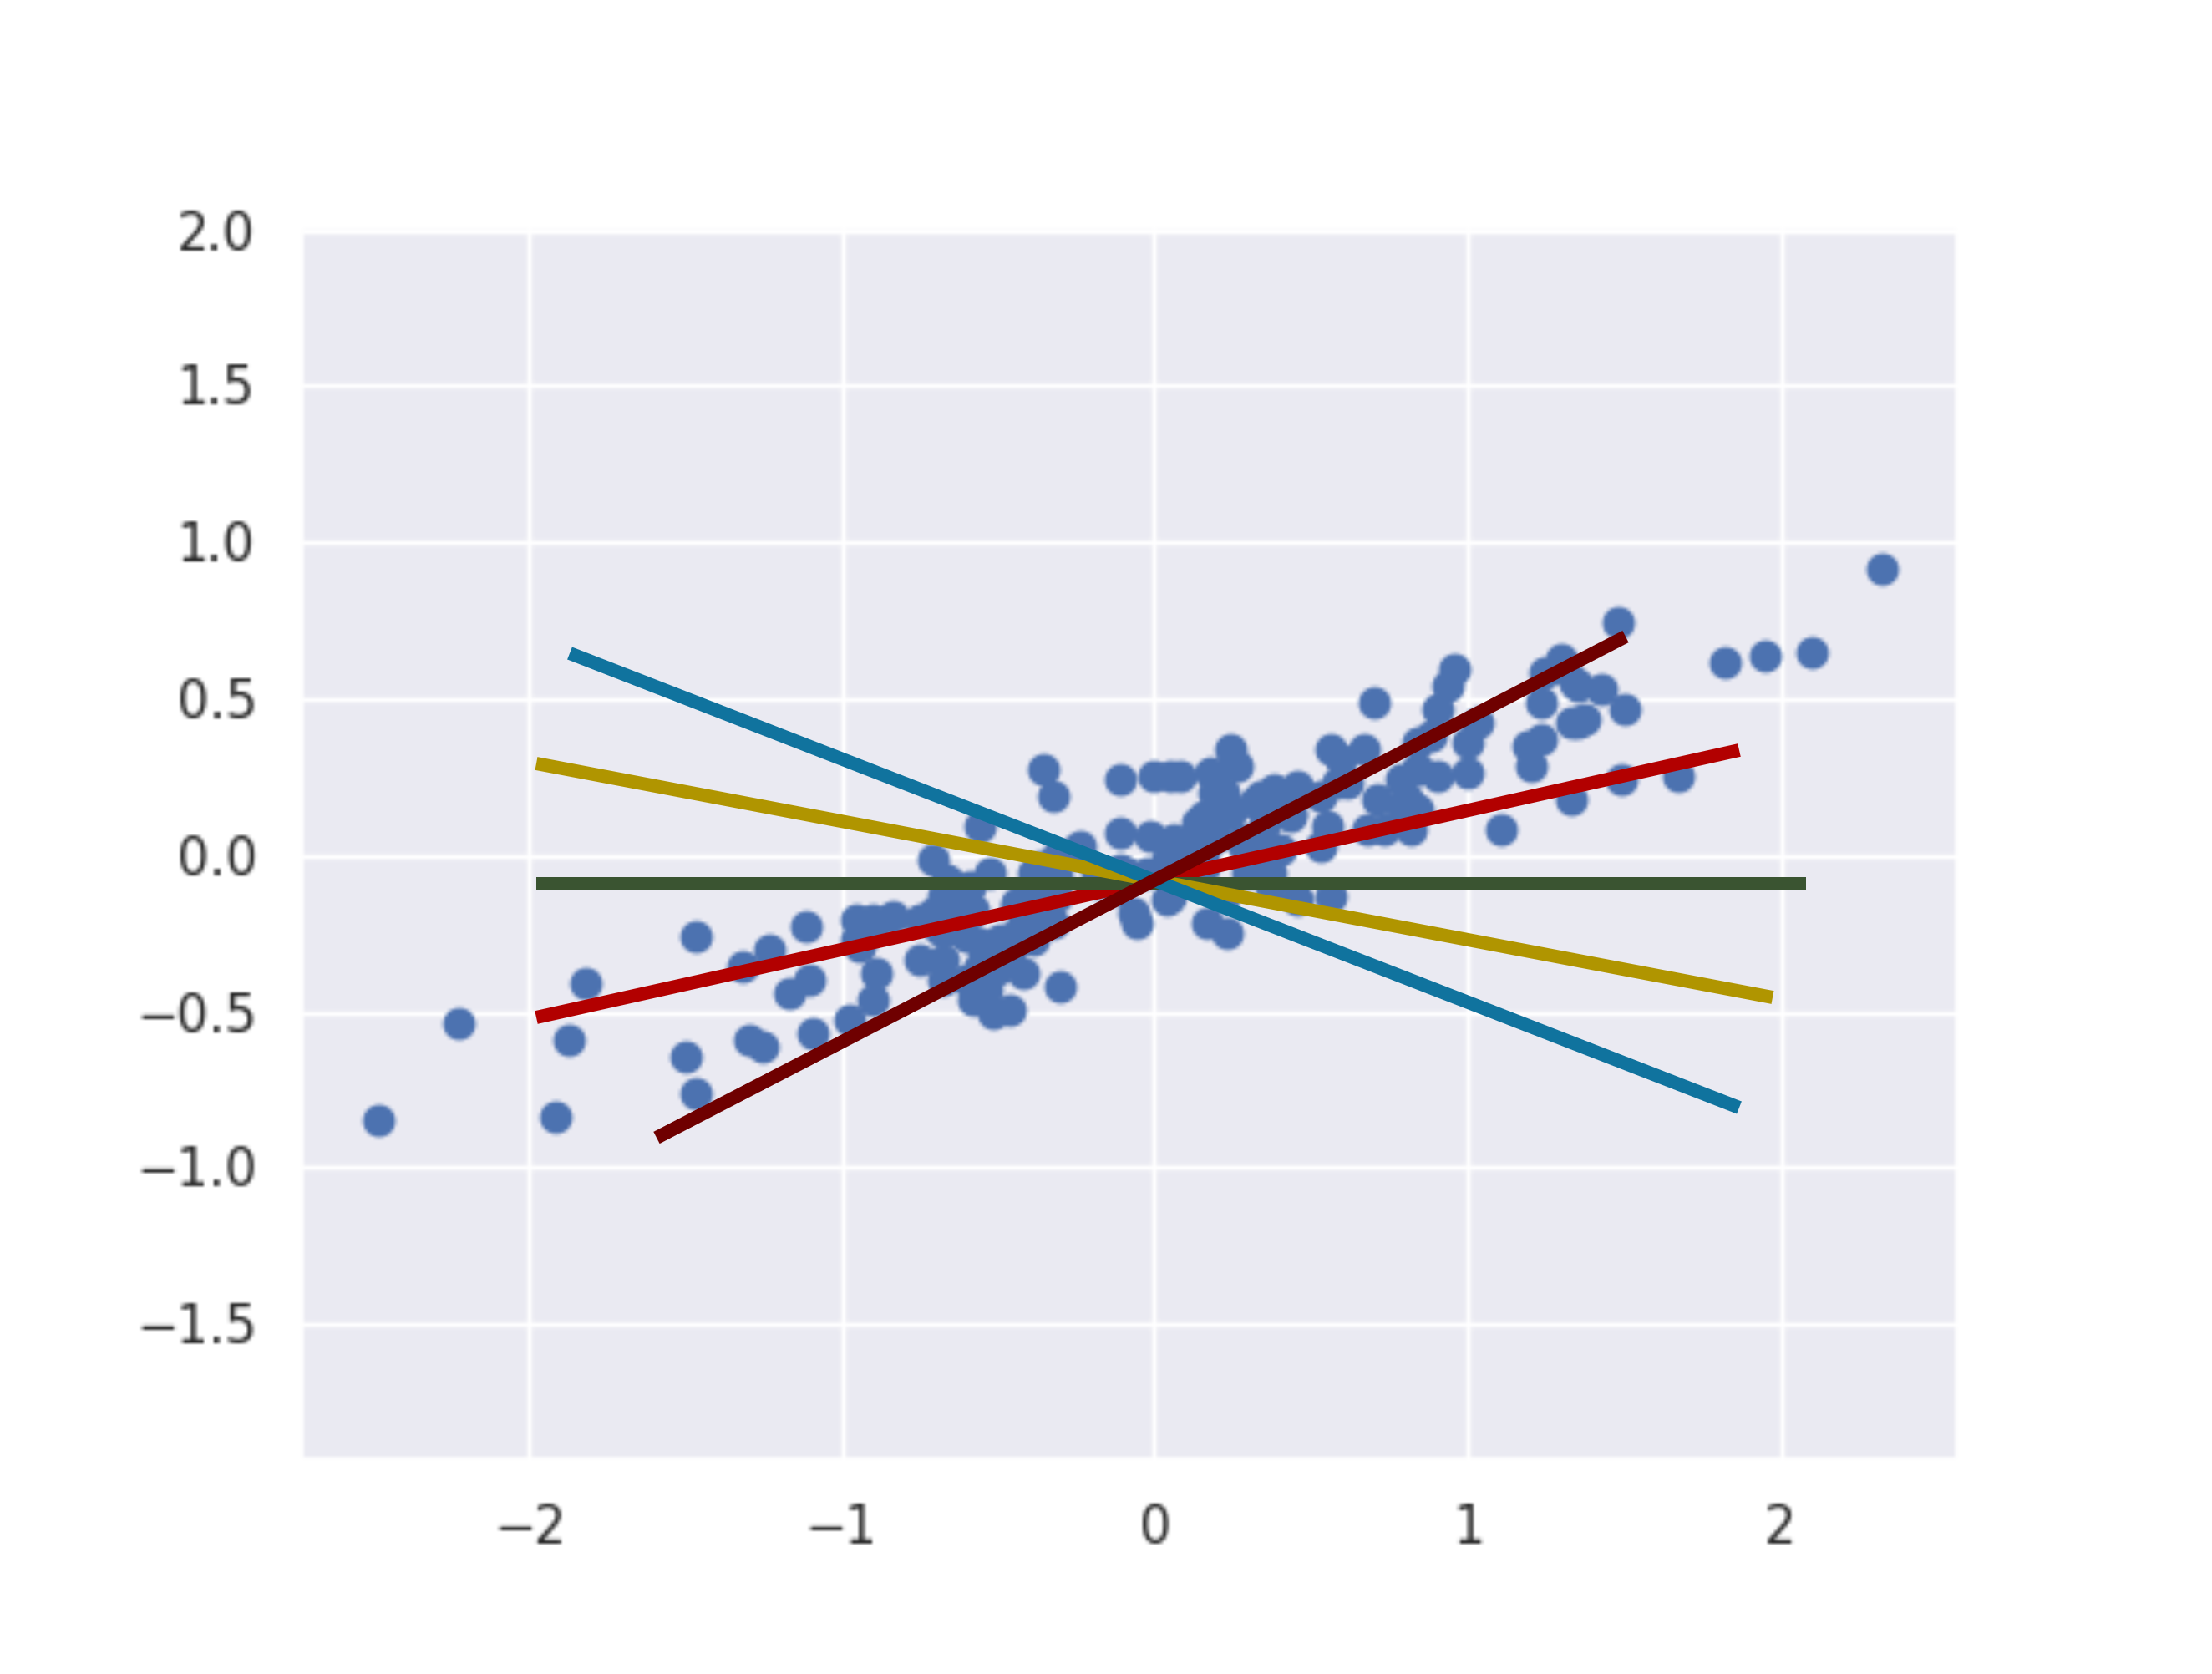
\includegraphics[width=9cm]{./pic/iVu9zQYG.png}
		      \caption{}
		      \label{fig:pca_vector_to_find}
	      \end{figure}
	      %
	      \newpage
	\item
	      圖 \ref{fig:two_vector_project}為部分資料集於兩向量上的投影示意圖,從圖 \ref{fig:pca_project_all}可以發現,資料於\(\vec{v}\)上的投影擁有較小的變異數。
	      \begin{figure}[h]
		      \begin{center}
			      \begin{tabular}{ccccccccccccc}
				      \subfigure[資料於\(\vec{v}\)上的投影 ]{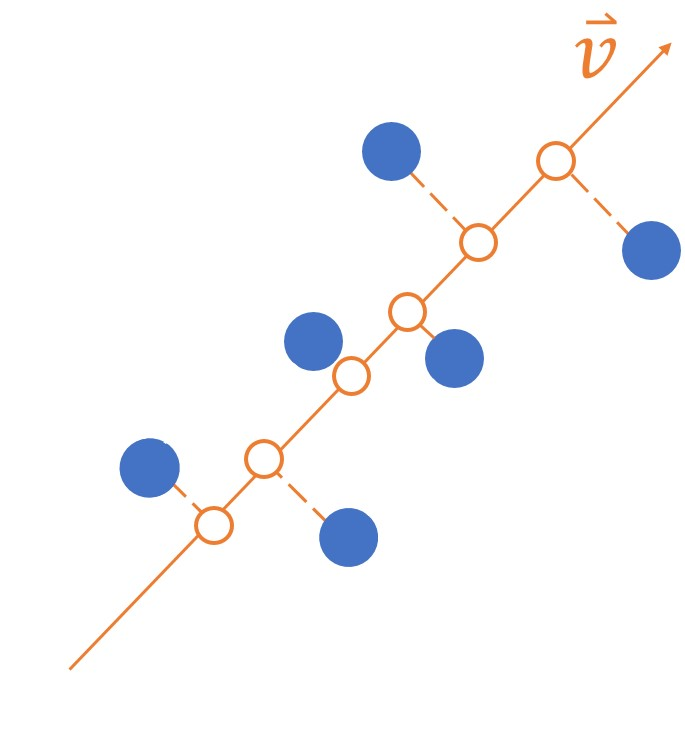
\includegraphics[width=5cm]{pic/pca_project_1.jpg}\label{fig:typeA} } \par &
				      \subfigure[資料於\(\vec{{v}'}\)上的投影]{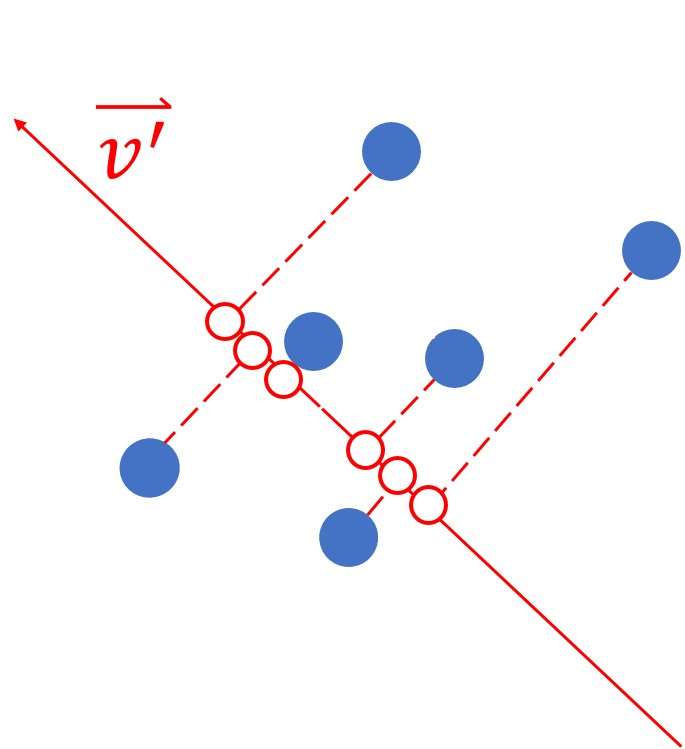
\includegraphics[width=5cm]{pic/pca_project_2.jpg}\label{fig:typeA} } \par \\
			      \end{tabular}
			      \caption{部分資料集投影於兩向量上示意圖}
			      \label{fig:two_vector_project}
		      \end{center}
	      \end{figure}

	      \begin{figure}[H]
		      \centering
		      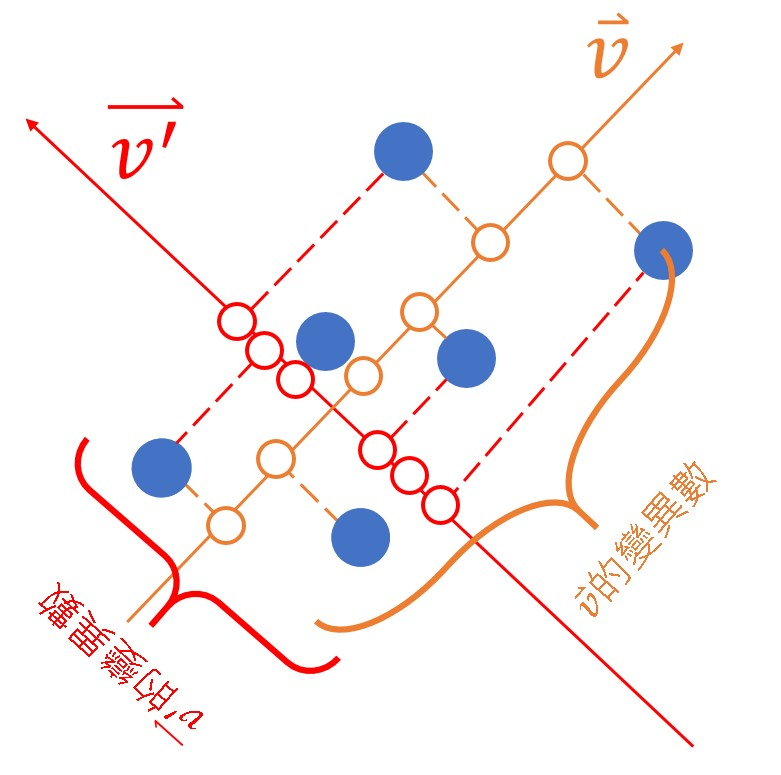
\includegraphics[width=6cm]{pic/pca_project_all.jpg}
		      \caption{\(\vec{v}\) 與\(\vec{{v}'}\)的變異數比較}
		      \label{fig:pca_project_all}
	      \end{figure}

	      %
	\item
	      此資料經過PCA的計算之後,我們可以得到比較有代表性的兩個特徵成份,較長的為PC1,較短的為PC2,如圖\ref{fig:pc1_and_pc2}所示,而變異量的值分別為0.7625與0.0184 。
	      \begin{figure}[H]
		      \centering
		      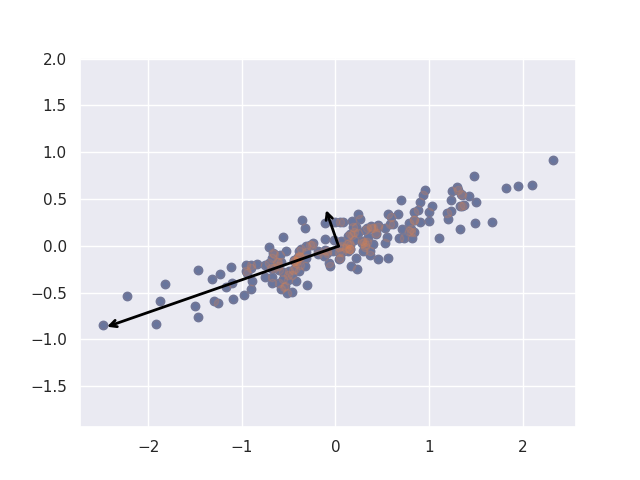
\includegraphics[width=9cm]{pic/pca_with_pca_axis.png}
		      \caption{}
		      \label{fig:pc1_and_pc2}
	      \end{figure}


	\item
	      圖\ref{fig:pca_transform}為資料集經過PCA轉換的結果,橫軸為PC1,縱軸為PC2,能從圖中與上面得到的變異量發現,PC1所函概的資訊足以代表整個資料集。進而將原本二維的資料,轉換成一維,作為模型訓練的輸⼊。


	      \begin{figure}[H]
		      \centering
		      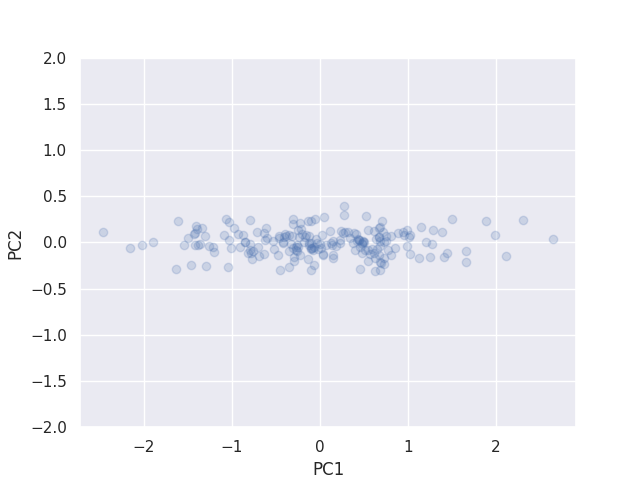
\includegraphics[width=9cm]{pic/pca_transform.png}
		      \caption{}
		      \label{fig:pca_transform}
	      \end{figure}

\end{itemize}


\section {結論}
從以上的舉例中,可以發現,經由PCA的轉換,我們可以分析出對於整個資料集最具代表性的成份,作為後序模型訓練的輸⼊。
也許二維的資料可能沒那麼明顯,但如果是影像資料(通常是具有高維度的資料),除了能夠有效的進行資料降維,提取影像中重要的特徵,還能因為維度的減少進而提高分類的運算速度。

